\section{Beta Decay}
\begin{figure}[ht!]
\centering
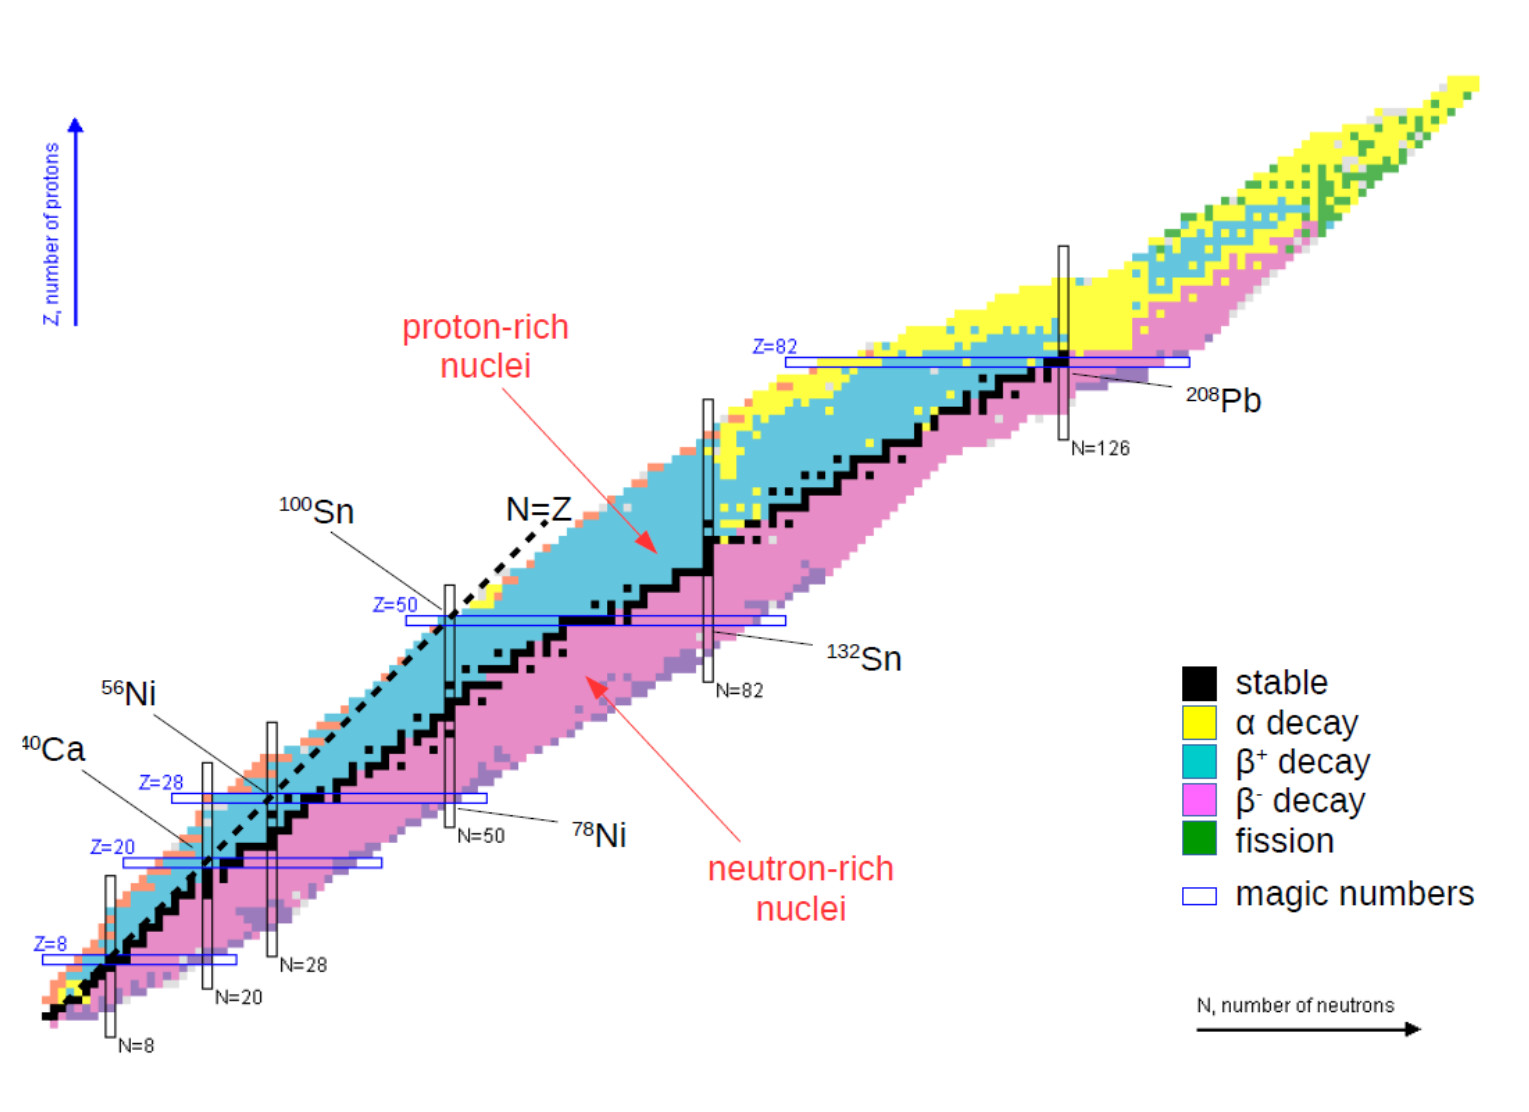
\includegraphics[width = \textwidth]{radioactive_nuclei_chart.png}
\caption{Beta decay is most popular with smaller nuclei.}
\label{fig: radioactive_nuclei_chart_2}
\end{figure}

\subsection{$β^{-}$ Decay}
\vspace{1mm}
\begin{wrapfigure}[7]{r}{0.45\textwidth}
\centering
\vspace{-12.5mm}
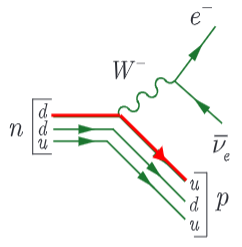
\includegraphics[width = .35\textwidth]{beta_minus_decay.png}
\caption{Feynman diagram of $β^{-}$ decay.}
\label{fig: beta_minus_decay}
\end{wrapfigure}
The neutron turns into a proton, electron and electron anti-neutrino. Only the electron and anti-neutrino are emitted. 
\begin{equation}
    n \rightarrow p + e^{-} + \bar{\nu}_{e} + Q_β
\end{equation}
This comes from the down quark turning into an up quark as seen in \cref{fig: beta_minus_decay}.



\vspace{12mm}
\subsection{$β^{+}$ Decay}
\begin{wrapfigure}[7]{r}{0.45\textwidth}
\centering
\vspace{-10mm}
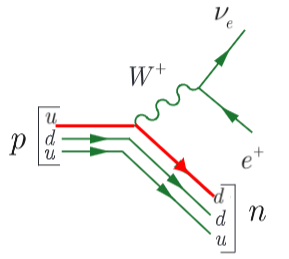
\includegraphics[width = .35\textwidth]{beta_plus_decay.png}
\caption{Feynman diagram of $β^{+}$ decay.}
\label{fig: beta_plus_decay}
\end{wrapfigure}
The proton turns into a neutron, positron and electron neutrino. Only the positron and neutrino are emitted.
\begin{equation}
    p \rightarrow n + e^{+} + \nu_{e} + Q_β
\end{equation}
This comes from the up quark turning into a down quark as seen in \cref{fig: beta_plus_decay}.


\vspace{10mm}
\subsection{Electron Capture}
\begin{wrapfigure}[13]{r}{0.45\textwidth}
\centering
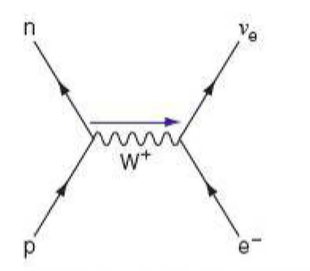
\includegraphics[width = .35\textwidth]{electron_capture.png}
\caption{Feynman diagram of electron capture.}
\label{fig: electron_capture}
\end{wrapfigure}

The nucleus captures an electron and turns a proton and electron into a neutron and electron neutrino. 
\begin{equation}
    p + e^{-} \rightarrow n + \nu_{e} + Q_β
\end{equation}
This comes from the up quark turning into a down quark. Only the neutrino is emitted as seen in \cref{fig: electron_capture}.

\vspace{10mm}
\subsection{Free Proton Decay}
\begin{itemize}
    \item A free proton can not decay. It will only decay inside the nucleus because of the binding energy, through beta decay and electron capture. 
    \item When decaying, the mass of the entire system is reduced. This cannot happen for a lone proton. 
\end{itemize}

\subsection{Energy Conservation}
\subsubsection{Neutron Decay}

We assume the neutron is at rest before the decay. 
\begin{equation}
    m_nc^2 = m_pc^2 + m_ec^2 + m_{\bar{\nu}_e}c^2 + K_{e} + K_{p} + K_{\bar{ν}}
\end{equation}
We define the $Q$-value:
\begin{equation}
    Q = \left(m_n - m_p - m_e - m_{\bar{ν}}\right)c^2
\end{equation}
Inserting the $Q$-value into the energy conservation equation:
\begin{equation}
    Q = K_{e} + K_{p} + K_{\bar{ν}}
\end{equation}
The recoil experienced by the proton is so small, as is the mass of the anti-neutrino. We tend to ignore both, giving:
\begin{equation}
    Q = m_n - m_p - m_e ≈ K_{e} + K_{\bar{ν}}
\end{equation}


\subsubsection{$β^{-}$ Decay}
We now consider the nucleus at rest before the decay.
\begin{equation}
  \ce{_{Z}^{A}\text{X}_{N}} → \ce{_{Z+1}^{A}\text{Y}_{N-1}} + e^{-} + \bar{\nu}_{e}
\end{equation}
The $Q$-value is derived from the nuclear mass $m_{N}$. We ignore the mass of the anti-neutrino. Nuclear masses is defined as follows:
\begin{equation}
  m\left(\ce{_{}^{A}\text{X}_{}}\right)c^2 = m_{N}\left(\ce{_{}^{A}\text{X}_{}}\right)c^2 + Zm_e c^2 - ∑_{i=1}^{Z} B_i
\end{equation}
\begin{equation}
  Q_{β^{-}} = \Big(m_{N} \left(\ce{_{Z}^{A}\text{X}_{}}\right) - m_{N}\left(\ce{_{Z+1}^{A}\text{Y}_{}}\right) - m_e\Big)c^2
\end{equation}
Adding the definition of the nuclear mass:
\begin{equation}
    Q_{β^{-}} = \Bigg[\Big(M\left(\ce{_{}^{A}\text{X}_{}}\right) - Zm_e\Big)- \bigg(m\Big(\ce{_{}^{A}\text{Y}_{}}\Big) - (Z+1)m_e\bigg) - m_e\Bigg]c^2 + ∑_{i=1}^{Z} B_i - ∑_{i=1}^{Z + 1} B_i
\end{equation}
Ignoring the binding energy of the electrons, we get:
\begin{equation}
  Q_{β^{-}} = \Big(m\left(\ce{_{}^{A}\text{X}_{}}\right) - m\left(\ce{_{}^{A}\text{Y}_{}}\right)\Big)c^2
\end{equation}

\paragraph{Example:}
Decay of $\ce{_{}^{210}\text{Bi}_{}}$ into $\ce{_{}^{210}\text{Po}_{}} + e + \bar{ν}_e$:
\begin{equation}
  Q_{β^{-}} = \Big(m\left(\ce{_{}^{210}\text{Bi}_{}}\right) - m\left(\ce{_{}^{210}\text{Po}_{}}\right)\Big)c^2 = 1.16 \text{ MeV}
\end{equation}
This sets an upper limit for the possible kinetic energy of the electron, and the energy of the anti-neutrino.
\begin{equation}
  K_{e_{\text{max}}} = E_{p_{\text{max}}} = Q_{β^{-}} = 1.16 \text{ MeV}
\end{equation}

\subsubsection{Electron Capture}
\begin{equation}
    \ce{_{Z}^{A}\text{X}_{N}} + e^{-} → \ce{_{Z-1}^{A}\text{Y}_{N+1}} + \nu_{e}
\end{equation}
\begin{equation}
  Q_{ε} = \Big(m\left(\ce{_{}^{A}\text{X}_{}}\right) - m\left(\ce{_{}^{A}\text{Y}_{}}\right)\Big)c^2 - B_n
\end{equation}
Where $B_n$ is the electron binding energy, depending on shell number $n$. Using conservation of energy we get:
\begin{equation}
    Q_{ε} = K_{\ce{_{}^{A}\text{Y}_{}}} + K_{\nu} ≈ K_{ν}
\end{equation}

This is a two-body decay, so the expected energy distribution is very sharp. As opposed to the three-body decay of $β^{-}$ decay, with a continuous energy distribution, as seen in \cref{fig: electron_energy_distribution}.

\begin{figure}[h!]
\centering
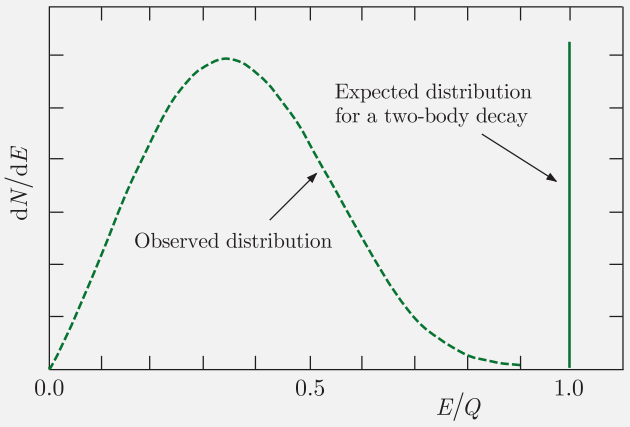
\includegraphics[width = .6\textwidth]{electron_energy_distribution.png}
\caption{Expected energy distribution for electrons in two-body and three-body decays.}
\label{fig: electron_energy_distribution}
\end{figure}

\subsubsection{Comparing Electron Capture \& $β^{+}$ Decay}
We have the $Q$-values for both processes:
\begin{equation}
    Q_{ε} = \Big(m\left(\ce{_{}^{A}\text{X}_{}}\right) - m\left(\ce{_{}^{A}\text{Y}_{}}\right)\Big)c^2 - B_n \quad , \quad  Q_{β^{+}} = \Big(m\left(\ce{_{}^{A}\text{X}_{}}\right) - m\left(\ce{_{}^{A}\text{Y}_{}}\right) - 2m_e\Big)c^2
\end{equation}
As $B_n ≪ 2m_ec^2$, we know that if a nucleus is able to undergo $β^{+}$ decay, has the energy to undergo electron capture. The opposite is not necessarily true. To undergo spontaneous $β^{+}$ decay, the $Q$-value must be equal or greater than $2m_ec^2 ≈ 1$ MeV. \\

The larger the $Q$-value the shorter the half-life. This is because the decay is more likely to happen if the energy released is higher.

\subsection{Fermi's Golden Rule}    
The decay probability $λ$ is constant and is given by:
\begin{equation}
  λ = \frac{1}{τ} = \frac{2π}{ℏ} |V_{fi}|^2 ρ(E_f)  \quad , \quad  V_{fi} = ∫ ψ^{*}_f V ψ_i dν
\end{equation}

\vspace{15mm}
It depends on: 
\begin{itemize}
    \item The density of the final state which decay can proceed. The higher the density, the faster the decay. 
    \item The matrix element describes the strength of the interaction, both strong and weak. 
    \item It Describes the overlap between the wave functions of initial and final states. The larger the overlap, the faster the decay occurs. 
\end{itemize}

\subsubsection{Fermi's Golden Rule for Decay}
These were points Fermi's theory had to address. 
\paragraph{Beta Decay:}
\begin{enumerate}
    \item Electron and neutrino do not exist before the decay process. The theory must account for their formation.
    \item Electron and neutrino must be treated relativistically. 
    \item The continuous distribution of electron energies must be reproduced by the theory (three body).
\end{enumerate}

\paragraph{Alpha Decay:}
\begin{enumerate}
    \item Alpha particle existed before the decay. 
    \item Alpha particle is treated classically.
    \item Alpha particle energy distributions monoenergetic (two body).
\end{enumerate}

\subsubsection{Fermi's Theory of Beta Decay}
Fermi introduced a small pertubation $V'$ to the state of the nucleus. This would have to be a weak interaction, compared to the strong interaction. This would explain why the decay is slow (seconds and longer), compared to the fast strong interaction. 